\chapter{METHODS}
\label{ch4:methods}

\section{Volume Registration Framework}

In the previous chapter, we discuss several techniques used to retrospectively correct motion. Motion correction pipelines may use denoising and filtering, but all pipelines begin with volume registration. In this section, we discuss a different approach to volume registration, how it compares to traditional volume registration, and how volume registration fits into a motion correction pipeline. 

%In this section, we discuss the two registration frameworks we apply to our rs-fMRIs: the traditional global volume registration framework and the DAG-based global volume registration framework. The registration frameworks will later be evaluated in comparison to each other, but will also be evaluated in the context of a complete motion correction pipeline. The motion correction pipeline of choice, ICA, will also be discussed in this section.

\subsection{Directed Acyclic Graph Based Volume Registration}

As discussed previously, the major drawback to Friston et al.'s approach to volume registration is that it only minimized the positional differences between the reference volume and the rest of the sequence. This drawback demonstrates an inability for the traditional approach to account for relationships in the patient's position throughout the scan. Intuitively, we know that the patient's position at any volume in the scan is more similar to his position in the immediately previous or subsequent volume than to another randomly chosen volume in the image.

In our proposed framework, we wish to account for these spatiotemporal relationships between temporally neighboring volumes in the sequence. To accomplish this goal, we start by viewing the rs-fMRI sequence as a directed acyclic graph (DAG). A DAG consists of a set of nodes and edges. Each edge has a direction associated with it and connects a pair of nodes. Since a DAG contains no cycles, there is no possible path back to a node once it has been traversed. 

\begin{figure}
\centering
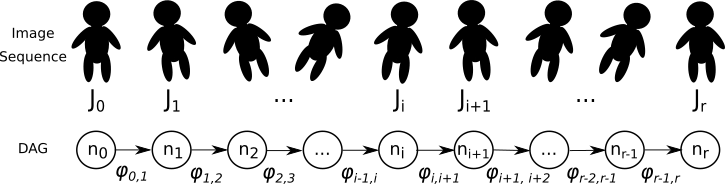
\includegraphics[width=.7\textwidth]{4/dag-chain.png}
\caption{A rs-fMRI can be viewed as a directed acyclic graph where each volume is a node and the edges connect from each volume $i$ to the following volume $i+1$.}
\label{ch4:fig:dag-chain}
\end{figure}

In the case of an rs-fMRI, each volume can be considered a node. The relationship between each pair of temporally neighboring volumes is represented as a directed edge connecting the node for the first volume to the node for the next volume. The acyclic nature of the DAG means that once a patient was in a specific position, he will never return to that exact same position with the exact same neurons firing. The position of the subject and his brain activity as measured by the BOLD signal may be similar in subsequent image volumes, but it will never be precisely the same. The perspectives of an rs-fMRI sequence as a set of images and of the sequence as a DAG can be seen in Figure \ref{ch4:fig:dag-chain}.

The cost of transitioning from one node to the next in our DAG has a parallel representation to the combination of the positional transformation needed to align volume $i$ to volume $i+1$ and the signal change between the volumes. This representation can be written as 

\begin{equation}
J_{i+1} = \phi_{i,i+1} J_i + \delta s_{i,i+1} + \epsilon
\end{equation}

\noindent{where $J_i$ and $J_{i+1}$ are volumes $i$ and $i+1$, $\phi_{i,i+1}$ is a matrix of transformation parameters that must be applied to $J_i$ to achieve the patient’s position in $J_{i+1}$, $\delta s_{i,i+1}$ is the natural change in BOLD signal, and $\epsilon$ is the change in BOLD signal due to motion. Currently, there is no way to estimate the natural change in BOLD signal and the change in BOLD signal due to motion without incorporating additional information about the MRI scanner and the patient that is not included in a rs-fMRI. We simplify our representation of the relationship between two volumes to}

\begin{equation}
J_{i+1} = \phi_{i,i+1} J_i + \epsilon^*
\end{equation}

\noindent{where $\epsilon^*$ is the change in the BOLD signal that cannot be accounted for after aligning the patient’s position in the two volumes. Here, we use the notation $\epsilon^*$ to represent the generic error change in BOLD signal across any pair of volumes.}

After aligning two volumes $i$ and $i+1$, we will then align volumes $i+1$ and $i+2$:

\begin{equation}
\begin{split}
J_{i+2} & = \phi_{i+1,i+2} J_{i+1} + \epsilon^* \\
& = \phi_{i+1,i+2} (\phi_{i,i+1} J_i + \epsilon^*) +\epsilon^*\\
& = \phi_{i+1,i+2} \phi_{i,i+1} J_i + \epsilon^{*'}\\
\end{split}
\end{equation}

Traditional volume registration assumes that 

\begin{equation}
\phi_{i,i+2} = \phi_{i+1,i+2} \phi_{i,i+1}
\end{equation}

\begin{figure}
\centering
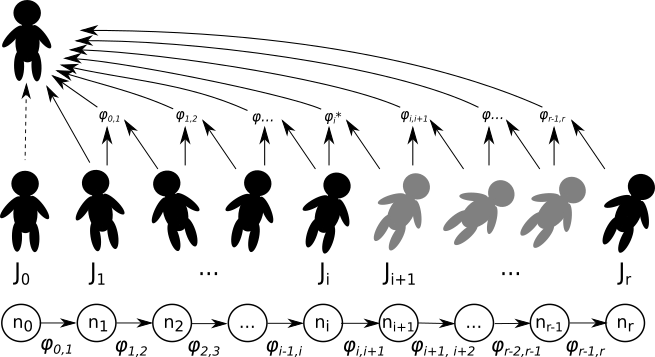
\includegraphics[width=.7\textwidth]{4/dag-registration.png}
\caption{The traditional approach to volume registration in an rs-fMRI sequence consists of registering all volumes in the sequence to a single reference volume.}
\label{ch4:fig:dag-reg}
\end{figure}

\noindent{and calculates $\phi_{i,i+2}$ directly. We argue that this assumption is not true in all cases. Rather than directly calculate $\phi_{0,i}$ and use it to align volume $i$ to the reference volume as the traditional method does, we calculate each component $\phi$ that is a factor of $\phi_{0,i}$. Each component $\phi_{i,i+1}$ is combined with the preceding $\phi_{0,i}$s to recursively align volume $i+1$ to the reference volume without making the large and often inaccurate transformations required by directly calculating $\phi_{0,i+1}$.} This process is outlined in Figure \ref{ch4:fig:dag-reg}.

\subsection{Motion Correction Pipeline}

Both the traditional and novel volume registration techniques were applied independently to each image from the subject cohorts described in Chapter \ref{ch:data}. After registration, three versions of each image existed: the original BOLD sequence, the sequence modified using traditional volume registration, and the sequence modified using the novel registration method.

The registration algorithms both used a combination of affine and nonlinear transformations to align each pair of image volumes. During the registration, the following registration parameters were used:
\begin{itemize}
\item Interpolation type: nearest neighbor
\item Number of threads: 100
\item Registration metric: cross correlation.
\end{itemize}

After performing volume registration to ensure the patient is in the same physical space throughout the image sequence, the image sequence may still contain artifacts due to motion. Our registered sequences underwent motion correction via a well-established motion correction pipeline. We chose to use the independent component analysis (ICA) pipeline outlined by Beckmann and Smith \cite{Beckmann2004}. The motion corrected sequences produced by MELODIC were saved alongside the original and registered sequences.  

\subsection{Implementation: Tools and Libraries}

The registration frameworks described in this section were implemented in Python using the nipype (Neuroimaging in Python Pipelines and Interfaces) library \cite{Gorgolewski2011}. Affine volume registration was performed using ANTs (Advanced Normalization Tools) \cite{Avants2014}. The metric used to estimate the dissimilarity between the pairs of volumes being registered was cross-correlation with a local window size of 5 voxels. 

The ICA pipeline described was applied to the registered images using FMRIB's MELODIC tool \cite{Beckmann2004}.

\section{Evaluating Registered and Motion Corrected Sequences Against Gold Standard Usability Thresholds}

The main goal of motion correction is to reduce the effects of motion on the image so that it is usable. The gold standards for rs-fMRI usability as established by Power et al. are that the FD and DVARs metrics must change less than 0.2 mm and 2.5\% normalized voxel units between at least 50\% of the neighboring volumes. The FD and DVARs metrics between each pair of subsequent image volumes were calculated for the original, registered, and motion corrected sequences. The metrics for each sequence were then compared to the gold standard image usability thresholds. This comparison answers the key question of how each registration framework impacts an established motion correction pipeline.

Additionally, a smaller comparison of the registered sequences was conducted. This comparison evaluates the immediate impact of the registration algorithm on the image sequence. It is highly unlikely that an entire image sequence would meet the Power et al. usability thresholds after only the initial step of a motion correction pipeline, but it is valuable to examine the impact of a volume registration algorithm at each stage of the pipeline. 

\textbf{Implementation.} We calculated the FD and DVARS metrics defined by Power et al. using the FSLMotionOutliers tool \cite{Power2012}. 

\section{Measuring Motion Patterns}

While the Power et al. usability thresholds for the FD and DVARs metrics quantify the volume-to-volume motion well, they do not quantify the overall motion contained in the image sequence. The FD and DVARs metrics as well as other imaging metrics can be used to compare every volume in an image sequence to every other volume in the image sequence to better quantify whole-sequence motion. As the FD and DVARs metrics have been discussed previously, we will focus in this section on three other image metrics: the Dice coefficient, the correlation ratio, and the mutual information. These five metrics were applied to each whole sequence to measure patient motion and image signal consistency throughout the entire scan.

\subsection{Dice Coefficient}

The Dice coefficient was proposed by Lee R. Dice in 1945 \cite{Dice1945}. Dice examined several existing metrics for measuring association, and finding them lacking, proposed his own ``coincidence index''. His coincidence index measures the association between a number of samples $a$ where condition $A$ is true and a number of samples $b$ where condition $B$ is true:

\begin{equation}
Index = \frac{2h}{a+b}
\end{equation}

In this equation, $h$ represents the number of samples where both conditions $A$ and $B$ are true. His index can take on any value between 1.0 and 0.0 such that a value of 1.0 means that conditions $A$ and $B$ are true for all samples. Similarly, a value of 0.0 means that conditions $A$ and $B$ are never both true for any sample. While this index is a count of samples that meant both conditions and not a true probability, Dice suggests that the chi-squared test can be used to determine if the combinations of conditions in the samples from a set of data is meaningful or due to random chance. 

Many medical imaging researchers have adapted the Dice coefficient to measure the overlap between pairs of images. %The images could be manual and automatic segmentations of the same area, segmented images registered to each other, or ELEPHANTS.
Zijdenbos et al. trained an artificial neural network to semiautomatically segment brain MRIs and compared the generated segmentations to manual segmentations using the Dice coefficient \cite{Zijdenbos1994}.
Zou et al. used the Dice similarity coefficient in their analysis of the reproducibility of manually segmented MRIs and the accuracy of automatic segmentations of the same images for prostate and brain tumor datasets \cite{Zou2004}. 
Liao et al. used it to measure the accuracy of a volume registration framework for aligning manual segmentations of multiple organs in fetal images \cite{Liao2016}. Bharatha et al. performed a study on pre- and intra-operative images of the prostate. They segmented the images, generated deformable finite element models of the segmentations, and used the Dice coefficient to compare the registered segmentations and finite element models \cite{Bharatha2001}.

It should be noted that the Dice coefficient as used in these contexts is a measure of similarity of items from two categories which take on binary conditions. Additionally, all studies mentioned in the previous paragraph require a manually segmented gold standard image to which the automatic segmentations or registered images can be compared. Medical images do not naturally have binary values, nor is it always reasonable to obtain manual segmentations of all images in a dataset. In cases where a good image segmentation cannot be obtained, other similarity metrics such as mutual information and cross correlation should be used instead.

\subsection{Correlation Ratio Matrix}

The correlation ratio is an asymmetrical, spatially informed measure of the overlap between images. It is different from other similarity metrices in that a lower correlation ratio indicates a better alignment between two images rather than a worse alginment. 

The earliest symbolic representation of the correlation ratio is 

\begin{equation}
\label{ch4:eq:cr-orig}
\eta = \frac{\Sigma}{\sigma_y} = \frac{\sqrt{\frac{\sum(n_x(\overline{y}_x - \overline{y})^2)}{N}}}{\sigma_y}
\end{equation}

\noindent where $n_x$ is the number of samples in any one set $x$, $\overline{y}_x$ is the average of the samples in $x$, $\overline{y}$ is the average of all samples in all sets, $\sigma_y$ is the standard deviation of all samples in all sets, and $N$ is the total number of samples across all sets \cite{Rugg1917}. The meaning of this equation was simplified by Ayres, who describes it as ``the ratio between two standard deviations'' \cite{Ayres1920}. In Equation \ref{ch4:eq:cr-orig}, the numerator is the standard deviation of a single set of samples with respect to all sets of samples, and the denominator is the standard deviation of all sets of samples. The process of calculating the individual components of this equation are outlined in \cite{Rugg1917}.

The correlation ratio was proposed for use in medical imaging applications in 1998 and compared to other similarity metrics. Roche et al. provide an example of algining two black images, one with a uniform gray stripe and the other with a horizontal gray gradient, such that the overlap between the two images is maximally similar \cite{Roche1998a}, \cite{Roche1998}. They show that the mutual information metric has a maximum value at every translation of an integer number of pixels while the correlation ratio had a maximum value at one single alignment. They apply the correlation ratio to MR images as well as computed tomography and positron emission tomography images. Their experiments suggest that in the context of multimodal registration, the correlation ratio balances accuracy and robustness.

In the context of medical imaging, the correlation ratio measures the functional dependence between a pair of images $X$ and $Y$. The correlation ratio of $Y$ given $X$ is

\begin{equation}
\eta(Y|X) = \frac{Var[E(Y|X)]}{Var(Y)}
\end{equation}

This equation is comparing the energy of $Y$ in $X$ to the total energy of $Y$. If $X$ and $Y$ overlap in area $\Omega$, the number of pixels in that area is $N = Card(\Omega)$. Since $X$ is known, it can be divided into sets of pixels $\Omega_i$ where each set is comprised of locations in $\Omega$ where the pixels $X$ have the same value $i$. 

Because the correlation ratio shows is a strong metric for measuring the similarity between two images, we suggest using it to quantify the similarity between all volumes in an image sequence. We choose to refer to this metric as the correlation ratio matrix. For a sequence of length $l$, the correlation ratio matrix $M$ is a square, asymmetrical matrix of size $l*l$. Each cell in $M$ is calculated as

\begin{equation}
M_{i,j} = \eta(J_i, J_j) = \frac{Var[E(J_i|J_j)]}{Var(J_i)} =  \frac{\sqrt{\frac{\sum |J_i|(\overline{J_i} - \overline{J_i \cap J_j})^2)}{|J_i \cap J_j|}}}{\sigma_{J_i \cap J_j}}
\end{equation}

\noindent where $J_i$ and $J_j$ are volumes $i \in l$ and $j \in l$ in the sequence, respectively, $|*|$ indicates the number of voxels in the operand, $\overline{*}$ indicates the average of the voxel values in the operand, and $J_i \cap J_j$ is the volume of space where images $J_i$ and $J_j$ intersect. %In volume registration, the computer assumes the entire contents of $J_i$ and $J_j$ intersect provided they are the same size (in voxels), which somewhat simplifies 

Since the matrix $M$ is quite large, using statistics describing $M$ rather than $M$ itself can simplify analyses. On the other hand, the whole matrix $M$ may be more comprehensively analyzed using statistical tests such as the $t$-test.

\subsection{Mutual Information}

The earliest description of mutual information was written in the context of mathematical theories behind networked communication \cite{Shannon1948}. Mutual information is a measure of the amount of information shared between two signals $X$ and $Y$. Specifically, mutual information measures how the joint distribution of the two signals compares to the marginal distribution of each signal \cite{Li1990}. It is a more general measure of dependence than correlation, which is limited to measuring linear dependence via a comparison of the marginal distributions. In terms of information theory, mutual information is represented as

\begin{equation}
\label{ch4:eq:mi_01}
MI(X, Y) = H(X) - H(X|Y)
\end{equation}

\noindent where $H(X)$ is the entropy of signal $X$

\begin{equation}
\label{ch4:eq:mi_02}
H(X) = - \sum_{x \in X} p_x log(p_x) 
\end{equation}

and $H(X|Y)$ is the conditional entropy of signal $X$ given the known signal $Y$

\begin{equation}
\label{ch4:eq:mi_03}
H(X|Y) = - \sum_{x \in X, y \in Y} p_{xy} log \frac{p_{xy}}{p_y}.
\end{equation}

Substituting Equations \ref{ch4:eq:mi_02} and \ref{ch4:eq:mi_03} in Equation \ref{ch4:eq:mi_01} produces the following

\begin{equation}
\label{ch4:eq:mi_04}
\begin{split}
MI(X, Y) & = - \sum_{x \in X} p_x log(p_x) + \sum_{x \in X, y \in Y} p_{xy} log \frac{p_{xy}}{p_y} \\
 & = \sum_{x \in X, y \in Y} p_{xy} log \frac{p_{xy}}{p_y} - 1*\sum_{x \in X} log(p_x) \\
 & = \sum_{x \in X, y \in Y} p_{xy} log \frac{p_{xy}}{p_x p_y}
\end{split}
\end{equation}

\noindent where $p(.)$ is the joint distribution of $X$ and $Y$, $p$ and $p$ are the marginal distributions of the two signals, and $X$ and $Y$ are the signals themselves. It is worth noting that since the two signals of interest are registered images, $x$ and $y$ refer to voxel locations in the same image space.

The mutual information can take on values in the range $[0, 1]$. A value of $0$ indicates that the two signals are completely independent and no information about signal $X$ is gained by knowing about signal $Y$. If signals $X$ and $Y$ are the same, 

Mutual information can be used to determine how the distribution of amplitudes in one signal relates to the distribution of another signal. It is commonly used in the medical imaging domain to objectively compare images of the same tissue taken using different modalities. For example, a computed tomography (CT) scan of a patient's abdomen contains different information about each tissue types' material properties than an MRI of the same organs. Some tissue types may appear similar in one of these modalities but drastically different in the other. Combining the information about a tissue's material properties gained from both imaging modalities provides more information than could be gained from either modality independently. (In other words, the resulting information is greater than the sum of its parts.)

Even though the rs-fMRIs in our study are all obtained using the same imaging modality, the spin history effects of patient motion can impact the recorded signal such that small changes in recorded BOLD signal are difficult to distinguish from noise due to motion. We choose to use mutual information to quantify to BOLD signal information across the entire image sequence.

\subsection{Implementation: Tools and Libraries}

To calculate metrics, we used several existing tools. 

As the Dice coefficient is a measure of the binary overlap of a pair of image volumes, it cannot be immediately applied to rs-fMRI volumes. The volumes first must undergo thresholding to separate voxels located within the brain and voxels in the background. The Dice coefficient could then be calculated for each pair of binary image volume. This calculation was implemented manually.

FLIRT (FMRIB’s Linear Image Registration Tool) was used to calculate the correlation ratio between each possible pair of volumes in the sequences \cite{Jenkinson2001} \cite{Jenkinson2002}. We then used the average and standard deviation of the correlation ratio distribution of each image to compare the images.

The mutual information calculation was implemented in two steps. The first step was to create a function that computes the joint histogram of the voxel value distributions between the two image volumes. This histogram was fed to a second function that converts the histogram counts to probabilities and calculates the mutual information value. 

\section{Patient Classification Using Motion Patterns} 

%Machine learning techniques can be used to classify images as belonging to different groups, but many of these techniques use difficult to interpret ``black box'' logic. In some cases, examining the logic behind a classification reveals patterns in a dataset which a human missed but a computer detected. These patterns can be helpful for improving human classification of the images, but they may also be based on artifacts which were not filtered out during preprocessing.

We suggest that the ways that patients move are specific to certain age groups. For example, fetal patients live suspended in amniotic fluid and as such are subject to different physical constraints than patients in other age groups. Neonatal patients are often scanned using a ``feed and bundle'' protocol, which often results in them sleeping through the scan. However, neonatal patients sometimes wake up during the scan, and the way a baby woken up from a nap moves is different from how a fidgety preadolescent moves. % though the terminology to define how the characteristics of these movement patterns differ is lacking. 

There is also a chance that patients within the same age group move differently possibly due to their cognitive state. Preadolescents who have ADHD likely become bored and fidgety in the MR scanner at different rates then their non-ADHD counterparts. Adults suffering from dementia may have more difficulty remaining still for the duration of a scan than adults from similar demographics with no dementia.

These patterns are essentially signals specific to different categories of patients. Machine learning techniques are useful for identifying patterns in signals from different sources. In addition to the motion metrics identified in the previous section, we will also use demographic and clinical data as features for our machine learning models. 

The goal of applying machine learning to identify population level motion patterns lends itself well to unsupervised machine learning techniques. Unsupervised learning techniques group samples from a population based on the patterns in their features. They do not use information about any known groups in the population to inform their classification processes. In this section, we discuss several different unsupervised machine learning techniques used to measure degrees of association within subgroups of a data set.

\subsection{K-means Clustering}

K-means clustering divides a group of data samples with $n$ features into $k$ groups based on each sample's distance from the average value of the group \cite{Hartigan1979}, \cite{macqueen1967}. In k-means clustering, the features of a set of data are viewed as the locations of each data sample in \textit{n}-dimensional space. In this space, \textit{k} cluster centroids are initially distrubuted. The distribution pattern can place the centroids either randomly between data samples or using randomly selected data points.

After the locations of the cluster centroids are initialized, the distance between each sample and each centroid is calculated. Each sample is assigned to the cluster represented by the centroid closest to it. Once the clusters are defined, the location of the centroid of each cluster is recalculated. The new centroid location is the mean of the locations of all samples in its cluster. The distance between each sample and each cluster centroid is recalculated, samples are reassigned to their closest cluster centroid, and the centroid of each cluster is recalculated. This process continues until a stopping criteria is fulfilled. With most unsupervised machine learning methods, the stopping criteria is that the classifications of the model do not change for a certain number of iterations. However, a maximum number of iterations is imposed on the learning process to prevent a model from running indefinitely. As a result, it is possible for a model to ``time out'' before reaching a stable state.

There are many variations of k-means clustering. For example, k-medians follows the same steps as k-means, but uses the median of the known data points in a cluster as the new centroid for that cluster \cite{Juan1998}. Another variation called k-mediods uses the data point closest to the center of the cluster as the new cluster centroid rather than a descriptive statistic of the cluster \cite{Kaufman1987}.

One of the major limitations of k-means clustering is that the number of clusters must be given to the model. It is difficult to know how many clusters are needed to adequately represent subgroups within a data set. If too many clusters are used, the groups identified by the algorithm will be more granular than they should be; however, using too few clusters will produce large groups which mask distinct subgroups. 



\subsection{Spectral Clustering}

While spectral clustering is related to k-means clustering, it approaches the problem of identifying associations in a group of data from a different perspective. Spectral clustering treats each data point in a sample as a node in a graph. The connections between data points are characterized by the adjacency matrix and the degree matrix of the graph. These two matrices are used to calculate the Laplacian matrix of the graph, whose properties are used to identify clusters. All three matrices are $n$x$n$ matrices, where $n$ is the number of data points in the sample. 

Herein, we discuss spectral clustering when the data can be represented using a simple graph. As such, certain mathematical shortcuts can be employed to simplify certain computations. A more general mathematical approach has been discussed by Ng, Jordan, and Weiss \cite{Ng2002}.

The adjacency matrix specifies the strength of the connection between the nodes represented by the rows and columns of the matrix. For data that does not begin in graph form, algorithms such as k-nearest neighbors can be used to generate the adjacency matrix. In the adjacency matrix, each entry $i, j$ contains the weight of the connection between node $i$ and node $j$. If the edges are unweighted, the value of the entry is either 0 or 1. If the graph is undirected, the value of entry $i, j$ is the same as the value of entry $j, i$. All entries where $i=j$ should be 0, unless node $i$ has a self-loop.

The degree matrix is a diagonal matrix which represents the number of edges connected to each node. If the graph is directed, the directionality of the degree matrix must be specified: a directed connection from node $a$ to node $b$ contributes to the count for node $a$ if the degree matrix counts the number of edges that begin at each node (outdegree), but contributes to the count for node $b$ if the degree matrix counts the number of terminating edges at each node (indegree). In the case of an undirected graph, the connections include all edges that begin or terminate at a node. To summarize, in an directed graph, each edge contributes to only one node count while in an undirected graph each edge contributes to both nodes.

The adjacency matrix and the degree matrix are used together to construct the Laplacian matrix of the graph. This calculation of the normal Laplacian for a simple graph (undirected and containing no loops) is straightforward: the adjacency matrix is subtracted from the degree matrix. The resulting matrix has the following properties:
\begin{itemize}
\item The diagonals are the number of connections per node less the number of self-connections
\item All off-diagonal values are the negative of the weight connecting node $i$ to node $j$.
\end{itemize}
It is important to note that if the graph in question contains loops or is directional, other methods must be used to calculate the Laplacian matrix. 

The Laplacian matrix can be used to explore many properties of a graph. In particular, the eigenvalues of the Laplacian matrix are informative about the number of connected components in the graph. Connected components are areas of the network that are connected to each other but not anything outside that component. Each connected component is not its own cluster, though: the connected components could be large and contain smaller sets of connected nodes that are good options for clusters.

To determine the number of clusters in the graph, the eigenvalues of the Laplacian matrix are sorted in increasing order. The number of zero-valued eigenvalues is the number of connected components in the graph. Eigenvalues close to zero suggest weak edges preventing some connected component from being two separate components. Manually examining these eigenvalues before performing spectral clustering can be informative about the number of clusters to create: the number of values below the first large gap between the eigenvalues are the number of clusters, $k$. The eigenvectors associated with these $k$ eigenvalues are used as a lower-dimensional representation of the data in the graph. Performing $k$-means clustering on this data produces the labels for the clusters within the data that are not linearly separable otherwise.

%\textbf{STRENGTHS AND WEAKNESSES}

\subsection{Agglomerative Clustering}

Agglomerative clustering is a specific type of hierarchical clustering which builds a tree of similarities between data samples from the ``bottom up'' \cite{Ward1963}. The data samples in agglomerative clustering are also viewed as distinct points in $n$-dimensional space, but the number of groups to identify is not specified. 

First, the distance from every data sample to every other data sample is calculated. The two data points that are closest together in terms of some similarity metric are combined into a single cluster. In the [relationship tree] representing the similarities between all data samples, a node is created and the joined data points are connected to that node. That node or cluster is treated as an intermediate data sample. The distance from the new ``data sample'' to every other data sample is calculated and the two closest data samples are again combined into another intermediate sample. A node representing the new cluster is added to the [relationship tree] and the data sample or samples merged into the cluster are connected to the node. The process of combining data points into clusters based on similarity to other data points terminates when all data points and clusters have been combined. 

The results of agglomerative clustering can be interpreted by traversing the [relationship tree]. The [relationship tree] recorded the history of which nodes were merged into which clusters at each stage. Due to the nature of agglomerative clustering, these stages can be viewed as distinct levels in the tree. Beginning at the final node (the root) of the tree, the granularity of the clusters can be explored. At the top level, there is only one cluster, but at the second to last level of the tree there will be two clusters, at the third level there will be three clusters, and so on. How each cluster grew can reveal information about the relationships between the data samples within that cluster.

%\subsection{Gaussian Mixture Models and Expectation Maximization}

%As the number of samples in a data set tends to infinity, the Central Limit Theorem states that the distribution of the data will approach a Gaussian distribution. Since our data is composed of different groups, it can be modeled as a collection of multivariate Gaussian distributions. The underlying Gaussian distributions would contribute to the overall distribution with different strengths. This type of model is called a Gaussian mixture model (GMM). The parameters defining the mixture models and their contribution to the overall distribution are unknown, but can be calculated using expectation-maximization.
%
%The goal of expectation-maximization (EM) is to estimate the maximum likelihood of parameters in statistical models. The EM algorithm is composed of two steps: the expectation step and the maximization step. During the expectation step, the logarithm of the likelihood of the parameters taking their current values is calculated. Then, during the maximization step, the values of the parameters are recalculated to maximize the likelihood in the next step. 
%
%The process of using the EM algorithm to estimate the parameters of a multivariate GMM begins with the initialization of the parameters for each multivariate Gaussian distribution. These parameters include the mean, the covariance, and the mixing coefficient of the distribution. 
%
%The EM algorithm may not find the globally optimal values of the parameters of interest. It is only guaranteed to find local optima. 

\subsection{Visualizing Clustering Results} 

The results of unsupervised clustering algorithms can be visualized to illustrate how the computer chose each group of samples. Depending on the number of features $n$ for each data sample, a dimensionality reduction method may be needed to transform the location of the data sample in $n$-dimensional feature space to a more easily visualized 2-dimensional or 3-dimensional space.

Dimensionality reduction methods include principle component analysis (PCA), TSNE, and XXXXXX.

Principle component analysis is a multivariate statistical technique that can be used to transform a set of variables with some degree of intercorrelation into a set of new, independent, orthogonal variables \cite{Abdi2010}. These variables are called principle components of the data set. The principle components are ordered with respect to the amount of variance in the data set that can be projected onto each component. In general, PCA fits an $p$-dimensional ellipsoid to a data set with $n$ features such that $p < n$. Each axis of the ellipsoid represents a single principle component. 

It is important to note that prior to the application of PCA, the data must be normalized. Normalizing the data allows different features to be compared on the same scale.

The first two or three principle components can be used to plot the results of a clustering algorithm in 2D or 3D space. An example of plotting clustering results using PCA can be seen in Figure [INSERT].

\textbf{TSNE}

Agglomerative clustering also lends itself well to visualization via heatmap. The heatmap allows the researcher to see the distribution of feature values across the dataset and across visually prominent clusters. ``Eyeballing'' a heatmap is no substitution for performing statistical analyses, but it can provide a better sense of context than summary statistics.  

\section{Predicting Patient Outcomes Using Motion Patterns}

In addition to examining the patterns of patient motion using unsupervised machine learning techniques, these patterns will also be used with supervised machine learning techniques to determine the relationship between motion types and clinical outcomes. In this section, we first present several supervised machine learning methods and then discuss more generally the limitations of supervised machine learning and the metrics we will use to evaluate our models.

\subsection{Regression}

The first supervised machine learning method we discuss is regression. In general, regression maps a set of features to a set of outcomes. Each feature is weighted based on its contribution to the outcome. Features which are more relevant to the outcome have larger weights, while less important features have smaller weights. 

The simplest version of regression is linear regression. Linear regression is used when the outcome being predicted has continuous values: a common example would be using the size of a house to predict its cost. The cost, $y$, would be modeled as

\begin{equation}
y = w_0 + w*x
\end{equation}

\noindent where $w$ is the weight assigned to the feature $x$, which is the size of the house, and $w_0$ is the weight for the bias in the model. As more features are added to the model, this equation generalizes to 

\begin{equation}
y = w_0 + \sum_{i \in N} w_i*x_i
\end{equation}

\noindent where $w_i$ is the weight for feature $i$, $x_i$ in the set of $N$ features. 

Alternatively, if the goal was to predict whether a house was owned or rented, linear regression would be a poor model choice. The goal of this problem is to identify a nominal class, not a value in a continuous interval. This type of problem is better suited for logistic regression.

Logistic regression takes the equation for linear regression and passes it through the logistic function. % BUT WHY
The logistic function is 

\begin{equation}
f(\pi) = \frac{1}{1+e^{\pi}}
\end{equation}

\noindent which means that a logistic regression models takes the form

\begin{equation}
y = \frac{1}{1+e^{(w_0 + \sum_{i \in N} w_i*x_i)}}
\end{equation}

This form of a logistic regression model is for binary, nominal outcomes, though multinomial logistic regression can model three or more outcomes and ordinal logistic regression can model ordered, discrete outcomes. For the purposes of this document, when we say logistic regression, we mean the form which models binary, nominal outcomes. 

%\textbf{STRENGTHS AND WEAKNESSES} 

\subsection{Support Vector Machine}

The mathematical framework for support vector machines (SVMs) was developed in 1963. In its original form, it could only be used to classify linearly separable data. SVMs treat data samples with $n$ features as points in $n$-dimensional space. The SVM is composed of a collection of binary hyperplane classifiers. Binary hyperplane classifiers label data as belonging to a class or not belonging to that class depending on which side of the hyperplane the data is located. For a single binary hyperplane, the ideal location and alignment of the hyperplane is calculated using the following equation

\begin{equation}
\vec{w}\cdot\vec{x}+b = 0
\end{equation}

\noindent where $\vec{w}$ is the vector of weights assigned to the features in $\vec{x}$ and the variable $b$ is a bias factor. This equation defines the hyperplane itself, but there are many hyperplanes that could satisfy this equation. The optimal hyperplane is determined using the support vectors. 

The support vectors are the data points closest to the hyperplane. They define the location and orientation of the hyperplane. The space between the points on opposite sides of the hyperplane is called the margin, $d$. The optimal hyperplane is defined as the hyperplane whose $\vec{w}$ and $b$ result in the largest $d$.

The largest $d$ occurs when the weights for the data samples are minimized. The weights indicate how important a data sample is in defining the hyperplane. Data samples which do not increase the size of $d$ (are not support vectors) should not contribute to the model. These samples should be assigned weights of $0$.

When the ideal $\vec{w}$ and $b$ parameters have been determined, data on one side of the hyperplane is labeled as belonging to one class while the data on the other side of the hyperplane does not belong to that class. In a two class scenario, data that does not belong to one class clearly must belong to the other class. As more classes are added to a data set, the number of hyperplanes must also increase. Instead of optimizing a single hyperplane, the entire collection of hyperplanes must be optimized together.

In some cases, data with $n$ dimensions may not be separable in $n$-dimensional space. In 1992, it was proposed that the original data could be mapped to a higher dimensional space where it would be linearly separable. The SVM could be built in that space and would still function as a linear classifier, even though it would appear to be a nonlinear classifier in the original space. Different kernel functions have been developed. 

After a SVM model has been trained, the kernel used to map the data from $n$-dimensional space to the higher dimensional space is used to map new data to that space. The new data is assigned labels depending on where it lies in the higher dimensional space.  

SVMs are versatile supervised learning techniques that perform well in classifying both linearly and nonlinearly separable data. By their very nature, they find the globally optimal solution. However, finding the optimal parameters for a SVM model can be a computationally expensive and complex process depending on the characteristics of the data samples.

\subsection{LSTM Recurrent Neural Network}

% And of course I would be remiss if I left out neural networks, the current sin du jour of supervised machine learning

One of the most popular supervised learning algorithms is the artificial neural network. A basic artificial neural network is composed of connected layers of units modeled after neurons in a biological brain. Every artificial neural network has at least two layers: an input layer and an output layer. The number of neurons in the input layer is the same as the number of features in the data being fed to the network. The input layer is connected to the output layer by weighted edges. For a network with $n$ features in the input layer and one neuron in the output layer, the value predicted by the network 
for data point $\vec{x}$ is given as

\begin{equation}
\label{ch4:eq:nn_01}
f(\vec{x}) = \vec{w} \cdot \vec{x} + b
\end{equation}

\noindent where $\vec{w}$ is the weight assigned to the edge connecting each input neuron to the output neuron, $\vec{x}$ is the values of the input vector, and $b$ is an offset factor.

Layers can be added between the input layer and the output layer to model more complex relationships. These layers are called hidden layers because they are not seen at the data input or model output. The value of each neuron in each layer can be calculated using the values of the neurons in the previous layer, which means that for two layers, Equation \ref{ch4:eq:nn_01} expands to

\begin{equation}
f(\vec{x}) = \vec{w_2} (\vec{w_1} \cdot \vec{x} + b_1) + b_2
\end{equation}

More generally, Equation \ref{ch4:eq:nn_01} can be written as

\begin{equation}
\label{ch4:eq:nn_02}
f_n(\vec{x}) = \vec{w_n} f_{n-1}(\vec{x})+ b_n
\end{equation}

\noindent where dot product of the weights of the current layer $w_n$ and the output $f_{n-1}(\vec{x})$ of the previous hidden layer $n-1$ are offset by some bias factor $b_n$ to produce the output $f_n(\vec{x})$ of the current layer. For the first layer of the network, the output is calculated using Equation \ref{ch4:eq:nn_01}.

To model nonlinear relationships in data, this equation must be generalized further to allow for activation functions. Activation functions are intended to represent the action potential firing in a biological neuron. A biological neuron is either activated or not activated, but the activation function of a neuron in an artificial neural network is not limited to binary states. For example, the output of a rectified linear unit (ReLU) is in the range $[0, \inf)$, a sigmoid function's output is in the range $(0, 1)$, and a hyperbolic tangent produces a value in the range $(-1, 1)$. Different activation functions are used for different applicationd depending on the desired behavior of the model.

We represent the activation function generically as $g_n(\cdot)$ and rewrite Equation \ref{ch4:eq:nn_02} as

\begin{equation}
\label{ch4:eq:nn_03}
f_n(\vec{x}) = g_c \left( \vec{w_n} f_{n-1}(\vec{x})+ b_n \right)
\end{equation}

Until this point, we have been describing feed-forward neural networks. All of the connections flow in a single direction from the input nodes to the output nodes. Networks built using a feed-forward paradigm are often used for pattern recognition or other cases where a given input is associated with a known output. However, neural networks can also have connections that skip layers, link back to previous layers, or connect to other neurons in the same layer. This type of network is called a recurrent neural network.

One particularly interesting type of recurrent neural network is a long short-term memory (LSTM) network. LSTM networks have more complex unit structure than basic neural networks. LSTM units are composed of a memory component and three types of gates: an input gate, an output gate, and a forget gate. The memory component tracks the current value of the unit. The input gate dictates how much data being passed to the cell impacts the memory component, the forget gate dictates how long a value is stored in the memory component, and the output gate dictates the impact of the value in the memory component is used to produce the output activation of the unit. Due to the nature of the LSTM units, networks made of LSTM units have an advantage over feed-forward networks when working with time-series data. 

%One of the major drawbacks of both regression and SVMs is that the data used to train these models must be in feature vector form. Neural networks have the ability to work with more complex input data. They have been used for tasks as complex as speech recognition and video processing. 


\subsection{Application of Supervised Machine Learning}

Generally, the outcomes of interest when applying supervised machine learning to medical data are some definition of normal and abnormal. We choose to perform two different analyses bases on two definitions of normal. 

The first definition of normal is that enough motion can be removed from the image that the image is usable. The abnormal label is that the image cannot be recovered based on the patient's motion patterns.

The second definition of normal is that the patient is healthy. We choose to identify the opposite label of ``the patient is healthy'' as ``the patient \textbf{may} not be healthy'' because of the heterogeneity of our data. CHD is a heterogeneous disease with many presentation types, and the neurodevelopmental disorders add another degree of granularity and complexity to a subject's clinical diagnosis. While it would be impressive to be able to build a clinical decision support tool that can diagnose a patient as having a particular form of CHD accompanied by a specific neurocognitive disorder, this goal is not the purpose of this project.

If a machine learning model reaches 100\% accuracy on both training and test data sets, data scientists should immediately assume something has gone wrong either with the model itself or with the training and testing data. Current machine learning models suffer from the difficulty of balancing two sources of error: bias and variance. Bias is the degree to which the machine learning model matches the underlying model of the training data. Variance is the breadth of the distribution of the data from the population of interest covered by the training data. Models with low bias and high variance overfit the training data: they model the training data well but generalize poorly to new data. Conversely, models with high bias and low variance underfit the training data: they fit the training data poorly, possibly because they learned noise in the training data rather than the signal. Underfitted models fail to capture the important signals from the training data and perform poorly overall.

A good model neither overfit nor underfits the training data. It has low bias and low variance, and the challenge of balancing these two sources of error has been discussed elsewhere but is important to address here to set realistic expectations about the training and testing classifications of a model. Ideally, the model will classify both training and testing data well, but it is not possible with current techniques and data availability for a model to have perfect classification of every data sample. 

The ``wellness''/``goodness'' of a binary classification model is determined using a truth table. A truth table is a $2*2$ table filled with the number of occurrences where data was classified correctly and incorrectly as belonging to each class. An example table can be seen in Table \ref{ch4:tab:truthtable}.

% Please add the following required packages to your document preamble:
% \usepackage{multirow}
\begin{table}[]
\caption{An example of a truth table for a binary classifier predicting the presence or absence of a condition.}
\label{ch4:tab:truthtable}
\begin{tabular}{cc|c|c|}
\cline{3-4}
\multicolumn{2}{c}{\multirow{2}{*}{}}                                                & \multicolumn{2}{|c|}{\textit{Actual}}               \\ \cline{3-4} 
\multicolumn{2}{c|}{}                                                                 & \textbf{Condition True} & \textbf{Condition False} \\ \hline
\multicolumn{1}{|c|}{\multirow{2}{*}{\textit{Predicted}}} & \textbf{Condition True}  & True Positive (TP)      & False Positive (FP)      \\ \cline{2-4} 
\multicolumn{1}{|c|}{}                                    & \textbf{Condition False} & False Negative (FN)     & True Negative (TN)       \\ \hline
\end{tabular}
\end{table}

Various metrics can be calculated from the truth table, such as sensitivity and precision. Sensitivity measures how well the model performed at correctly identifying actually true data samples:

\begin{equation}
sensitivity = TPR = \frac{TP}{TP+FN}
\end{equation}

\noindent Precision measures the ratio of positive predictions to actually true data:

\begin{equation}
specificity = PPV = \frac{TP}{TP+FP}
\end{equation}

These metrics are also known as the true positive rate and the positive predictive value, respectively

These metrics are independently informative about different aspects of the model, but during training only one metric is used to evaluate a model's performance. Accuracy, for example, is a measure of how many data samples were classified correctly:

\begin{equation}
A = \frac{TP+TN}{TP+TN+FP+FN}
\end{equation}

We choose to use the balanced F1 score to evaluate the success of our supervised learning models. The balanced F1 score is calculated as:

\begin{equation}
\begin{split}
F1 & = \frac{2 \cdot TPR \cdot PPV}{TPR+PPV} \\
& = \frac{2 \cdot TP}{2 \cdot TP + FP + FN}
\end{split}
\end{equation}

The balanced F1 score places equal value on a model correctly identifying actually true data compared to false data as well as identifying as much actually true data as possible. Accuracy only accounts for the number of correctly classified data samples. In cases where all classes in a data set are not evenly represented, the balanced F1 score produces a more robust model than accuracy. 


\section{Describing Motion Patterns}

In previous sections we describe practical knowledge about how fetal, neonatal, preadolescent, and adult patients move in different ways during MRI scans. We wish to quantify these movement patterns using the metrics described earlier in this chapter and identify appropriate terminology that can be used to describe them.


%\subsection{Demographic-Related Motion Patterns} % in different populations to formally describe age-group or clinical status related motion patterns.

%The purpose of this experiment is to address the following questions. Are there any patterns in motion that are similar (a) within age groups, (b) within groups scanned at the same site, or (c) within broad clinical groups? Are these patterns due to spurious signals?

%To ensure that there are no confounding signals in our datasets, we first use unsupervised machine learning techniques to identify correlations between subject images and their demographic data. The techniques we will use are several types of clustering (agglomerative, k-means, and spectral) as well as principle component analysis (PCA) and regression. Features of the images before and after registration will be used as training data for each model and different demographic features will be used as the true classes. %The demographic data for each subject includes the subject's age at the time of scan, gender, race, dominant hand, and scan site. (NOTE: THAT SENTENCE IS FOR MULTISITE STUDY DATA, NEED TO SPECIFY, ALSO NEED TO GET ALL CLINICAL DATA.)

%\textbf{Phantom Images.} The phantom images are included in this analysis, though no significant results are expected other than potential site specific results.

%\textbf{Clinical Cohorts.} Any demographic features which influence the division of patients into groups will be reported and accounted for during later analyses. After identifying and accounting for demographic groups, we will expand the analysis to clinical and behavioral outcomes.


%\subsection{Clinical-Related Motion Patterns} %Employ machine learning techniques to (a) measure the impact of motion on image harmonization in multi-center studies, and (b) evaluate the relationship between motion and cognitive, clinical, and behavioral outcomes of CHD patients.

%In addition to evaluating the effects of the DAG-based framework within the context of a motion correction pipeline, the registered images are used to explore the relationship between motion and clinical outcomes. Unsupervised machine learning techniques such as agglomerative clustering and k-means clustering are applied to the data. The results of the clustering techniques elucidate whether there are patterns in motion specific to certain patient groups. These groups could include patients with similar clinical outcomes, patients from the same site, or potentially other clinical or demographic groups.

%\textbf{Machine Learning for Optimal Motion Correction} Start with a classification module for identifying severity of motion between template volume, previous volume(s), and current volume. The classifications will be based either on the patterns identified in Aim 2, or on the positional and signal change differences between the volumes of interest.

%After the severity of the motion reflected in a volume is determined...

%\textbf{Aim 4: Does Motion Correction Recover True Signal?} Hinted at earlier in first section of chapter, should it get its own section?